%%%%%%%%%%%%%%%
% Related Work and Background %
%%%%%%%%%%%%%%%

\section{Typology of Urban Forms}
To best understand the concept of road network patterns, one has to consider the urban forms of cities that best shape the road network patterns within such cities. Based on the literature on historic and more recent urban forms (for example, [\cite{deKlerk:1980} \& \cite{Rottier:1980}], identified six different forms (figure \ref{fig:urban forms})).
\begin{figure}[h]
\centering
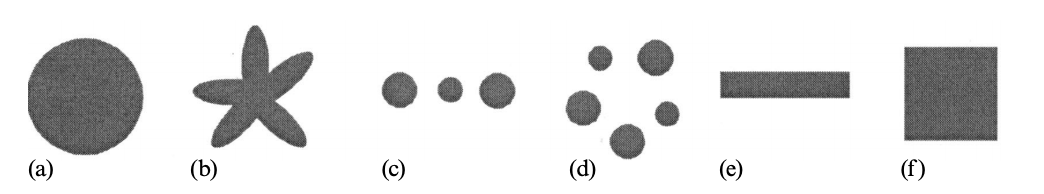
\includegraphics[width=0.95\textwidth,center]{picture/figure1.png}
\caption[Morphological Urban Forms]{Morphological urban forms: (a) the concentric city, (b) the lobe city, (c) the linear polynuclear city, (d) the concentric polynuclear city, (e) the linear city, (f) and the grid city.  Source: \cite{deKlerk:1980} \& \cite{Rottier:1980}}
\label{fig:urban forms}
\end{figure}

The concentric city as defined by [\cite{Snellen:2002}] is a typical form of a city that grew from a small (historic) center along a series of radial exit roads. The spaces between the radial roads have been filled in over time, thus giving the city its concentric shape. This city shape is frequently associated with a radial road network based on historic routes, but it can also be combined with ring or grid networks. These cities are often quite compact, with a strong center and a mixed supply of facilities.

The lobe city on the other hand has an history that is quite similar. The main distinction observed is that the city has grown between some radial roads but not others. The lobe shape can be caused by roads extending in some directions or by the form of deliberate city planning.[\cite{Snellen:2002}]

According to [\cite{Snellen:2002}],  the linear polynuclear and concentric polynuclear cities share several similarities between them. These cities' morphologies can often develop in two very different ways. Either a number of smaller settlements close to each other begin to function as one city, or a city is specifically designed to be polynuclear. Almere, the only true polynuclear city in the Netherlands, is best described as a concentric polynuclear city.

The linear city can be thought of as an extreme form of the city form. These cities frequently have a grid-type transportation network for cars, but this is not always the case.[\cite{Snellen:2002}] 

Grid cities is considered to be the collective noun for cities with a more or less rectangular shape. [\cite{Snellen:2002}].

In the selection of locations for data collection, both the linear and grid cities were included.[\cite{Snellen:2002}]

\section{Road network patterns}
The complexities of shape and structure set road patterns apart from many other objects of urban or transport analysis. For example, road width is merely a linear quantity and traffic flow is a simple ratio (vehicles per hour). Even the issue of density boils down to a straightforward ratio, however fiercely the significance of different numerators or denominators may be contested. By contrast, there is no straightforward or standard descriptor that is used to capture road patterns. 

However, without an adequate description of the pattern or structure, it will be difficult to compare structures across cases – identifying patterns that are 'good' or 'bad' for different purposes – and thus make robust, generalizable recommendations for urban layout design.

In the literature, several approaches are used to classify the road pattern in an urban area. One common approach is based on [\cite{Marshall:2005}] concept's of macroscopic and microscopic street networks developed by. The Macro-level or Citywide Street network distinguishes streets that are generally continuous across a significant portion of the city and probably service travel from one part of the city to another and, in many cases, trips to or from the city. Because these streets are on routes that are not continuous across a significant portion of the city, the Micro-level or Neighborhood Street network generally serves residential neighborhood travel. [\cite{Marshall:2005}] used two types of Neighbourhood Street networks (tree and grid) to describe a city's street hierarchy [\cite{Marshall:2010, Marshall:2011}]. 

Another common approach focuses directly on the overall street pattern in a community rather than focusing on the different types of streets and then combining them to form a pattern. [\cite{Southworth:2003}], for example classified street patterns into five categories: gridiron, fragmented parallel, wrapped parallel, loops and lollipops, and lollipops on a stick. Figure \ref{fig:streetpatterns} depicts their classification.

\begin{figure}[h]
\centering
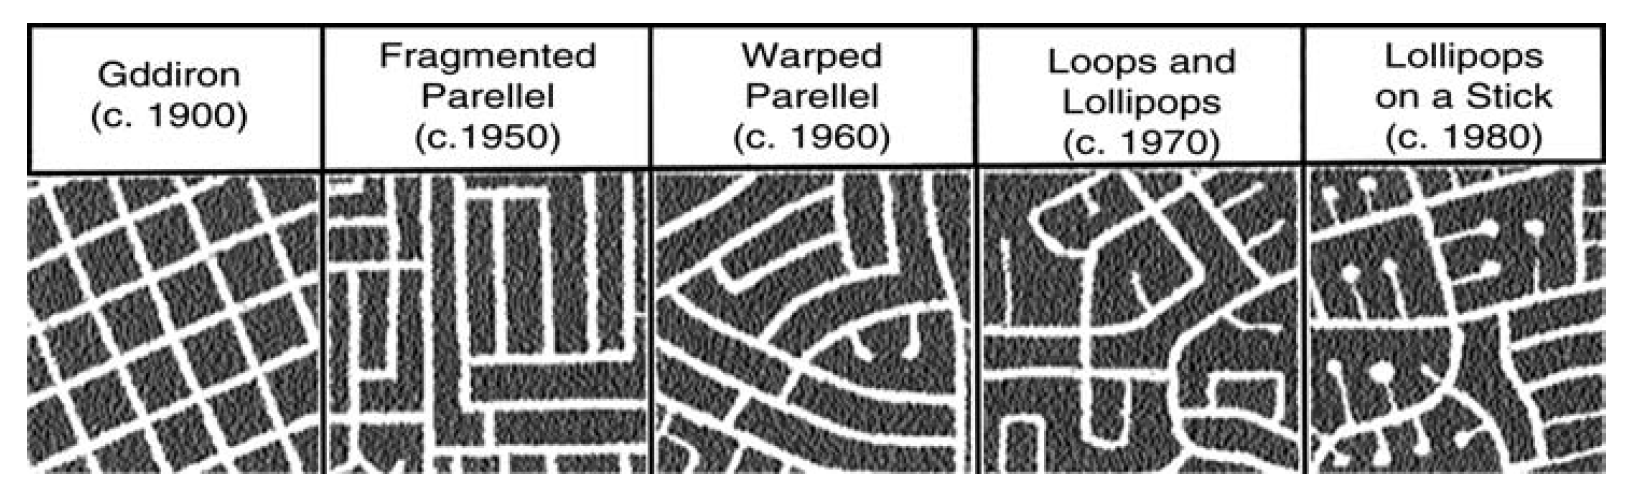
\includegraphics[width=0.95\textwidth,center]{picture/figure2.png}
\caption[Types of Street Patterns]{Types of street patterns. Source: \cite{Southworth:2003}}
\label{fig:streetpatterns}
\end{figure}

The typology (form or pattern) of the city itself is a major influencing factor on road network patterns. [\cite{Snellen:2002}] research on the urban form, road network type, and mode choice for frequently performed activities in the Netherlands is very useful in identifying different road network types. They distinguished six major urban forms, as defined by [\cite{deKlerk:1980, Rottier:1980}], namely the concentric city, the lobe city, the linear polynuclear city, the linear city, and the grid city. They identified five basic networks based on these six principles. Figure 2.33 depicts their classification. Because this approach is one of the foundations for the classification scheme used in this study, a brief description of each will be provided.

The radial network is suitable for all transportation modes. For example, in the Netherlands, it is the classic network for urban public transport, where buses radiate to and from the city center or railway station. When used as a network for the other transport modes, it offers direct accessibility to the city center. This network type, however, is prone to congestion issues. It can, in theory, be applied to all morphological urban forms. [\cite{Snellen:2002}]

\begin{figure}[h]
\centering
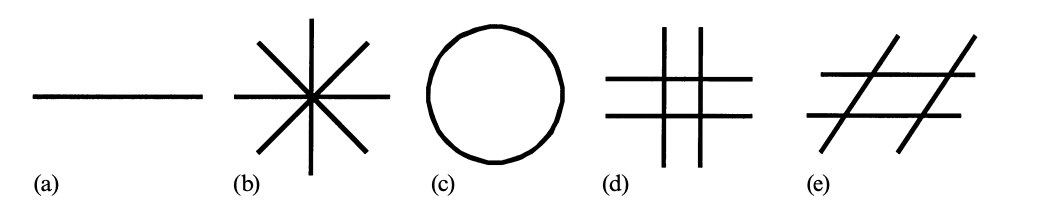
\includegraphics[width=0.95\textwidth,center]{picture/figure3.png}
\caption[Elementary Transportation Networks]{Elementary transportation networks: (a) the linear network, (b) the radial network, (c) the ring, (d) the grid, and (e) the shifted grid. Source: \cite{Snellen:2002}}
\label{fig:transportnetworks}
\end{figure}

The ring network is commonly used as a network for motorized transportation. It allows for the concentration of a large amount of traffic on a single road while relieving other areas of traffic congestion. City centers, in particular, are frequently encircled by a ring structure. This network type is not commonly used for public transportation in medium-sized cities, despite the fact that it would provide good connections between city districts while avoiding trips to and from the city center. This network type can be applied to all morphological urban forms for both motorized and nonmotorized transportation. This network type is ideal for public transportation in concentric polynuclear cities. [\cite{Snellen:2002}]

The (shifted) grid network is simple and direct, provides numerous route options, and disperses traffic across many streets. The numerous road crossings in the system are disadvantages of this network type. It is primarily used for both motorized and non-motorized transportation. This network type is flexible in theory and can be applied to all morphological urban forms. [\cite{Snellen:2002}]

Another approach to defining toad network pattern is that of [\cite{Chan:2011,Lima:2015}]. In their research, they divided a specific road network into four basic street network styles, as shown in figure [\ref{fig:transportnetworks}]. The patterns seen in their results are common in cities and correspond to the real-world design requirements of a street network. Their approach is one of the pillars of the classification scheme used in this study, and each will be briefly described below.

\begin{figure}[!ht]
\centering
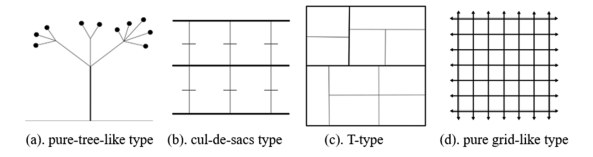
\includegraphics[width=0.75\textwidth,center]{picture/Cul de.png}
\caption[Abstract Structures of Four Kinds of Urban Street Networks]{Abstract structures of four kinds of urban street networks. Source: \cite{Han:2020}}
\label{fig:transportnetworks}
\end{figure}

Pure tree-like network pattern (Figure \ref{fig:transportnetworks}a). There are apparent backbone roads throughout the region and T-type cross and end-roads, forming a low-connected level network structure. This type of street network helps to protect residents' privacy and traffic stability, but it may be less robust than others. [\cite{Chan:2011,Lima:2015,Han:2020}]

The cul-de-sacs network pattern (Figure \ref{fig:transportnetworks}b). There are several trunks that run through a region with numerous end-roads. This type of network has good accessibility, but may be weaker in terms of interior connectivity than others. [\cite{Chan:2011,Lima:2015,Han:2020}]

T-type network pattern (Figure \ref{fig:transportnetworks}c). Though this street network resembles a pure grid-shaped network, the T-type intersections may improve trunk transportation efficiency while potentially decreasing connectivity. [\cite{Chan:2011,Lima:2015,Han:2020}]

Pure grid-like network pattern (Figure \ref{fig:transportnetworks}d). Despite being more connected than the others, transportation efficiency is typically lower due to the high number of intersections and short distances between them. [\cite{Chan:2011,Lima:2015,Han:2020}]

\section{Graph Networks}
In its most basic form, a network is a collection of points connected in pairs by lines. \cite{Newman:2010} "Network data structures for geographic information science (GIS) are methods for storing network data sets in a computer to support a variety of network analysis procedures," according to [\cite{Curtin:2008}]. To name a few network applications, a network can represent a transportation or communications system, a utility service mechanism, or a computer system" [\cite{Curtin:2008}]. Flow networks and pure networks are two types of networks. According to Fischer, flow networks contain information about the flow of something within a network, whereas a pure network represents any network's overall structure, with the topological relationships being the primary concern. [\cite{Ficsher:2003}]. Computer networks, social networks, transportation networks, and other types of networks are also examples of networks. The concept that a network, by definition, can be used to model and analyze linear features and their relationships is critical.

Networks, network models, and network analysis are based on mathematics, typology, and graph theory [\cite{Sovik:2014}]. The following section discusses important contributions from graph theory that provide the foundation for characterizing networks, network analysis, and network pattern analysis.

A graph is an abstract representation of a set of elements and the connections between them [\cite{IntroductiontoGraphTheoryTrudeau:1994},\cite{Boeing:2017}]. A graph is made up of the following G = (N,E). In this example, G is the graph, and the elements N are interchangeably referred to as nodes (points) or vertices, with the connections E referred to as edges (lines) or links. For the sake of consistency, this study employs the terms nodes and edges. The number of nodes within the graph (referred to as the graph's degree) is usually represented as n, while the number of edges is usually represented as m. Two nodes are adjacent if they share an edge, two edges are adjacent if they share the same node, and a node and an edge are incident if the edge connects the node to another node. A model like this is frequently depicted as a picture. Figure \ref{fig:directedgraph} shows an example of a simple graph with three vertices and three edges. Vertices, in general, do not loop back on themselves [\cite{Duo:2002}].

\begin{figure}[h]
\centering
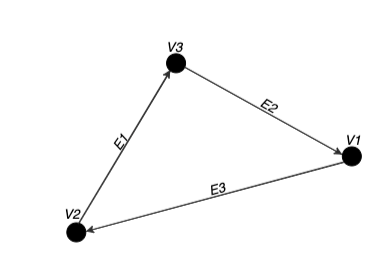
\includegraphics[width=0.95\textwidth,center]{picture/figure5.png}
\caption[Directed Graph]{Directed Graph}
\label{fig:directedgraph}
\end{figure}

The edges of an undirected graph point in both directions, whereas the edges of a directed graph, or digraph, point in only one direction (i.e., edge E2 points from node V3 to node V1, but there is not necessarily a reciprocal edge V3,V1). A self-loop is an edge that connects one node to another. Parallel (i.e., multiple) edges between the same two nodes are also possible in graphs. Multigraphs, or multi digraphs if they are directed, are the name given to such graphs. An undirected graph is said to be connected if any node can be reached from any other node. A digraph is weakly connected if the graph's undirected representation is connected, and strongly connected if any node can be reached from any other node. A path is an ordered sequence of edges connecting some other ordered sequence of nodes. If two paths share no nodes other than end points, they are internally node-disjoint. The edges of a weighted graph have a weight attribute that quantifies some value between connected nodes, such as importance or impedance. The number of edges in the path between two nodes is the distance between them, whereas the weighted distance is the sum of the weight attributes of the edges in the path. [\cite{Boeing:2017}]

In 1736, Leonhard Euler published the first known example of problem solving using graph theory. In his seminal paper, he solved the Königsber Bridge Problem using a graph. In his writings, he sought a solution to the use of seven bridges connecting two islands to the banks and each other. The issue was crossing each bridge only once without going back. Interestingly, he demonstrated that there was no solution to the problem using graph theory [\cite{Duo:2002}]. 

Since Euler's time, graph theory and its implementations have evolved. Today, network modeling is often based on the same underlying concepts used by Euler, but with the introduction of computers and GIS, the amount of knowledge that can be modeled and the complexity of the networks have grown. Social networks (in which individuals are nodes and their interpersonal connections are edges) and the World Wide Web are well-known examples (where web pages are the nodes and hyperlinks leading from one to another are the edges). A complex network (the configuration and arrangement of its nodes and edges) has a non-trivial topology, which means that the topology is neither completely regular nor completely random. The majority of large real-world networks are dynamic [\cite{Newman:2010}]. In this analysis, complex spatial networks [\cite{OSullivan:2014}], i.e. complex networks with nodes and/or edges embedded in space, are of particular importance. A street network, like railways, power grids, and water and sanitation networks, is an example of a dynamic spatial network with nodes and edges embedded in space [\cite{Barthelemy:2011}]. The paper "The Structure and Role of Complex Networks," by [\cite{Newman:2003}], is recommended for a more in-depth review.

\section{Road network as Graphs}
Road networks are typically represented as graphs, with nodes representing intersections and dead ends and edges representing street segments that connect them [\cite{Barthelemy:2008, Cardillo:2006, Lin:2013, Marshall:2018, Porta:2006}]. These edges are embedded in space and have length and compass bearings [\cite{Barthelemy:2011}]. The current study uses undirected nonplanar multigraphs to model urban street networks with potential self-loops. Though most faithfully guided graphs reflect flow restrictions (such as vehicular traffic on one-way streets), undirected graphs best model urban structure by referring to street segments (i.e. the linear sides of city blocks) by a factor of one. Although many street networks are roughly planar (with very few overpasses or underpasses), nonplanar graphs provide more detailed models by accommodating certain bridges and tunnels that also occur [\cite{Boeing:2018, Eppstein:2008}].

The data used to study these networks is typically derived from digitized street shapefiles. Individual local, state, or federal entities can generate data in each country, but the criteria for digitization and data availability vary. As a result, cross-sectional street network orientation and entropy analysis have been limited to specific geographic areas or to small samples [\cite{Boeing:2019}]. However, OpenStreetMap now provides a new alternative data source. OpenStreetMap is a global collaborative mapping project that includes highways, houses, services, and other geographic features. Although the quality of its data varies by country, its street data is generally of high quality, particularly in cities [\cite{Barrington-Leigh:2017, Barron:2014, Zielstra:2013}]. The OpenStreetMap data source allows for cross-sectional research into the shape and layout of street networks all over the world. Recently, researchers investigated the order and disorder of the street network using circuity and orientation entropy. Circuity focuses on street curvature measurements and how they apply to other urban network patterns [\cite{Boeing:2019, Giacomin:2015, Levinson:2009}]. The orientation entropy quantifies and visualizes the entropy of street orientations to determine their order [\cite{Courtat:2011, Gudmundsson:2013, Mohajeri:2013, Mohajeri:2013:1, Mohajeri:2014, Mohajeri:2012}]. [\cite{Louf:2014}] investigated the geometry of city blocks around the world as a function of block size and form factor, grouping them together to define the differences between US and European cities. However, little is known about cross-sectional patterns in the spatial orientation and ordering of global road networks. This thesis builds on previous research into circuitry, order, and entropy by analyzing cities around the world and looking for similarities in their patterns and relationships using OpenStreetMap data.

A spatial network is planar if it can be represented with its edges intersecting only at nodes in two dimensions. For example, a road network may be planar (especially in some small scales), but most road networks are non-planar due to grade-separated expressways, overpasses, bridges, and tunnels [\cite{Boeing:2017}]. In spite of this, a large number of existing quantitative analyses of urban street networks represent them as planar graphs for tractability [\cite{Barthelemy:2008, Buhl:2006,Cardillo:2006, Masucci:2009, Strano:2013}], since bridges and tunnels are comparatively rare (in some places), so the networks are roughly planar. However, this oversimplification of tractability planarity can be needless and may cause methodological problems. The street networks mentioned so far are known as primal graphs that represent nodes as intersections and edges as street segments. This thesis, however, focuses on primal graphs because they preserve all the geographical, spatial, and metric information essential to the urban form and design that dual representations discard for a  street network as all the such as the length, shape, circuity, width, etc. The primal graph, on the other hand, represents all the spatial characteristics of a street network. Using Primal graphs may be a better approach to analyzing spatial networks where geography matters, since the physical space underlying the networks themselves contains the relevant information that cannot exist in the topology of the network alone [\cite{Ratti:2004}].

\subsection{Evaluation Metrics of Road Networks}
Road network topology is defined as the spatial arrangement of roads at a given location [\cite{Rodrigue:2016}]. It is conventionally evaluated by the measures of gridness, treeness, ringness, webness, [\cite{Barthelemy:2011, Buhl:2006, Gudmundsson:2013, Xie:2007}] and typology [\cite{Louf:2014}]. Recent advances in topology, graph theories and the growth in computing ability has paved the way for more advanced methods for quantitative analysis of road network patterns [\cite{Jiang:2004, Cardillo:2006, Bavelas:1948}].

In their research, [\cite{Xie:2007, Levinson:2012}], pointed out that the two fundamental structures commonly observed in the planar transport network include the tree-like network and grid-like network. In this regard, [\cite{Noda:1996, Tini:2018}] introduced the grid-tree-proportion index (GTP index) as a new mathematical measure uniting the alpha and gamma indices used to jointly evaluate the grid pattern, tree pattern, and other road network patterns that do not belong to either of the two categories highlighted [\cite{Usui:2011}]. The approach is also used to quantify the formation, coherence and connectivity of road network patterns [\cite{Gogoi:2013, Usui:2011, Wang:2017}]. In addition, it is used to assess the efficiency of traffic flow or movement in the road network. The GTP index ranges from the lowest value of 0 to the highest value of 1. The GTP index coefficient is computed by substituting the following formula.

\begin{equation}
{GTP}=\frac{e-V+1}{\left(\sqrt{V-1)^{2}}\right.}
\end{equation}

Where:
GTP $=$ Grid Tree Pattern
$\mathrm{e}=$ Total number of edges (Links)
$\mathrm{V}=$ Total number of vertex (Nodes)
{Source: \cite{Tini:2018}}

Road networks considered to be primal, non-planar, weighted multi-digraphs with self-loops can be characterized, described and evaluated by both metric and topological measures. Extended concepts and algorithms can be found in [\cite{Newman:2010, Barthelemy:2011}]. 

The metric structure, which is measured in terms of length and area, represents common transportation variables [\cite{Cervero:1997, Ewing:2010}]. [\cite{Boeing:2017}], defined the major density metrics as "average street length, mean edge length (in spatial units such as meters) in the undirected representation of the graph, which all act as the linear proxy for block size and show how fine-grained or coarse-grained the network is." Node density is defined as the number of nodes divided by the network's coverage area. The node density of a group of nodes with more than one street emanating from them is referred to as the intersection density (excluding dead-ends). The edge density is the sum of all edge lengths divided by the area, while the physical street density is the sum of all edges in the graph's undirected representation divided by the area." [\cite{Boeing:2017}]. All of these density measures provide additional information about the network's fine-grainedness. Finally, the average circuity is calculated by dividing the sum of all edge lengths by the sum of the great-circle distances between the nodes incident to each edge [\cite{Giacomin:2015}]. This is the average ratio of the edge's length to the straight-line distance between the nodes it connects.

Topological measures of the structure of a street network often indicate the configuration, connectedness, and robustness of the network as well as how these characteristics are distributed. The average node degree, or mean number of edges that are incident to each node, quantifies the connectivity of each node on average. “Similarly, but more precisely, the average streets per node measures the mean number of physical streets emanating from each intersection and dead-end. This adapts the average node degree to the physical form rather than to the directed circulation” [\cite{Boeing:2017}]. The statistical and spatial distributions of the number of streets per intersection describe the type, prevalence, and dispersion of the connectivity of all intersections in the network. Connectivity measures the minimum number of nodes or edges to be removed from a connected graph in order to disconnect it. It is considered to be a measure of resilience, since complex networks with high connectivity offer more routing options for agents and are more robust to failure. However, node and edge connectivity is less effective for approximately planar networks like street networks: most street networks will have the connectivity of 1, because the presence of a single dead-end means the removal of just one node or edge can disconnect the network [\cite{Boeing:2017}]. More usefully, the average node connectivity of a network the mean number of internally node-disjoint paths between each pair of nodes within the graph represents the expected number of nodes that has to be removed to disconnect a randomly selected pair of non-adjacent nodes [\cite{Beineke:2002}]. As [\cite{OSullivan:2014}] explains, both spatial integration and approximate planarity greatly limits a network’s distance, degrees and connectivity. Other measures of connectedness within a network such as intersection density, node degree distribution, and centrality/clustering (discussed in the next paragraph) can better capture the nature of a street network's connectedness than node or edge connectivity. Low connectedness networks can have several single points of failure, making the system especially vulnerable to perturbation. This is evident in urban design by the way of permeability and choke points, for instance, traffic jams can occur and circulation networks can fail if circulation within the network is forced through single points of failure. [\cite{Hajrasouliha:2015}] linked connectedness to pedestrian volume within a street network.

In addition to being able to better capture the nature of the connectedness of a road network than node or edge connectivity, clustering measures also show the topological structure and distribution of a street network. Boeing 2017, describes a node’s clustering coefficient as “the ratio of the number of edges between its neighbors to the maximum possible number of edges that would exist between these neighbors”. The weighted clustering coefficient is used to calculate the connectivity and complexity from how thoroughly the neighborhood of a given node is connected together, since it weighs the connectivity and complexity ratio from edge length and the average clustering coefficient as the mean of the clustering coefficients of all the nodes in the network. The weighted clustering coefficient was extended to neighborhoods within an arbitrary distance by [\cite{Jiang:2004}] to make it more applicable to urban street networks. The importance of nodes in a network is indicated by the Centrality. [\cite{Barthelemy:2004}], describes the Betweenness centrality as the evaluation of the number of shortest paths that pass through each node or edge. The maximum betweenness centrality in a network specifies the  proportion of shortest paths that pass through the most important node/edge [\cite{Boeing:2017}]. This is a measure of resilience: networks with a high maximum betweenness centrality are more vulnerable to failure if the single choke point fails. The average betweenness centrality is the mean of all the betweenness centralities in the network [\cite{Barthelemy:2011}]. In their work, [\cite{Barthelemy:2013}] used the betweenness centrality to identify top-down interventions against the bottom-up self-organization and evolution of Paris's urban network pattern. Closeness centrality represents, for each node, a reciprocal sum of the distance from that node to all other nodes in the network: that is, nodes rank as more central if they are on average similar to all other nodes. Finally, PageRank, developed by [\cite{Brin:1998}] is the algorithm used by Google to rank web pages. The PageRank algorithm is known to be a variant of the network centrality, namely the eigenvector centrality. PageRank can also be extended to street networks, as it ranks nodes on the basis of the structure of incoming links and the rank of the source node. [\cite{Agryzkov:2012, Chin:2015}]

\section{Graph Similarity Measures}
As a result of the recent developments on graph matching, different algorithms have been proposed to solve the problem of comparing graph-based representation [\cite{Bunke:2000}] . Though little has been explored in this regard for road network representations, these graph matching algorithms can be adapted in order to support the calculation of similarities. The following sections highlight some of the most important measures. It is also important to emphasize that there is no single criteria for selecting best measure because their performance is highly dependent on the characteristics of the graph [\cite{Papadimitriou:2010}]. As a result, experimentation is the best way to find the best algorithm for the problem at hand [\cite{Jouili:2010}]. 

These following descriptions below aren't comprehensive descriptions of every graph comparison method in use today, but they do show some similarities between them.

\subsection{Graph Edit Distance / Graph Isomorphism}
Graph isomorphism is one method for evaluating graph similarity. If two graphs are isomorphic, they are similar [\cite{Pelillo:1999}], or one is isomorphic to a subgraph of the other , or they contain isomorphic subgraphs. The drawback of graph isomorphism is that the exact versions of the algorithms are exponential, making them unsuitable for today's large graphs [\cite{Koutra:2011}]. The graph edit distance is a variant of the graph isomorphism problem, in which the goal is to transform one graph into another by performing a series of operations (additions, deletions, substitutions of nodes or edges, and reversions of edges). This method assigns a cost to each operation and seeks to find the operation sequence that will minimize the cost of matching the two graphs.[\cite{Koutra:2011}]

GED (graph edit distance) is a more flexible similarity measure that contemplates the differences in edges and nodes as well as the set of associated weights [\cite{Gao:2010}]. There are many adaptations of GED; however, the use of the bipartite variation of GED to limit algorithm complexity has been used as much as possible [\cite{Manrique:2018}]. 

The most basic graph distances and extensions aggregate element-by-element comparisons between the adjacency matrices of two graphs; [\cite{Golub:2013, Jaccard:1901, Hamming:1950, Gao:2010, Wallis:2001}]; because these methods are known to explicitly depend on the node labeling scheme (and are therefore not invariant under graph isomorphism [\cite{Chowdhury:2017}], their utility when comparing graphs with unknown labels  may be limited (e.g. graphs sampled from random graph ensembles). Several measures collect empirical distributions [\cite{Carpi:2011}] or a “signature” vector [\cite{Berlingerio:2012}] from each graph and compute the distance between them (using the Jensen-Shannon divergence, Canberra distance, earth mover’s distance, and other measures [\cite{Emmert-Streib:2016}], which allows for the comparison of graphs with different sizes. [\cite{Bagrow:2019}].

\subsection{Signature Similarity}
Signature similarity [\cite{Papadimitriou:2010}] is another graph similarity metric to consider. Using the node weights, the method attempts to generate a signature vector of 1s and 0s for each graph. The vectors are then compared by counting the number of matches between them. It normalizes the result and provides similarity measurements between 0 and 1.

\subsection{Spectral Distance}
Another approach is comparing the spectral properties of certain matrices characterized by graphs [\cite{Jurman:2015}], such as the non-backtracking matrix [\cite{Torres:2019, Mellor:2019}] or Laplacian matrix [\cite{Jurman:2011}], which is known as spectral distance. The relevant spectral properties associated with these distances are invariant under graph isomorphism. [\cite{Chowdhury:2017, vanSteen:2010}]. Some of these graph distance measures have been proven to be metrics (that is, they satisfy properties like triangle inequality, etc.) [\cite{Deza:2009}], while others have not.

\subsection{Feature-based Distance}
One method for comparing graphs is to look at specific "features" of the graph, such as the degree distribution, betweenness centrality distribution, diameter, number of triangles, number of k-cliques, and so on. Consider the vector as an empirical distribution and use the sample moments as graph features for vector-valued graph features (such as degree distribution) (or quantiles, or statistical properties). A feature-based distance compares graphs by comparing these features.

All of the methods discussed thus far are, of course, feature-based in general; however, in the special case where the features occur as values over the space V V of possible node pairings, they are frequently referred to as matrix distances. Similarly, if the feature under consideration is the spectrum of a specific matrix realization of the graph, the method is known as a spectral distance.[\cite{Wills:2020}]

[\cite{Berlingerio:2012}] proposes NETSIMILE, which is a feature-based distance with the  focus on local and egonet-based features (e.g., degree, volume of egonet as fraction of maximum possible volume, etc.). When k features are used, the method generates a feature-vertex matrix of size k n. The associated feature matrix generated is then reduced to a "signature vector" (a process referred to as "aggregation" by the authors of [\cite{Berlingerio:2012}] that consists of the mean, median, standard deviation, skewness, and kurtosis of each These signature vectors are then compared to determine the distance between graphs.

Feature-based methods for comparing graphs are popular in the neuroscience literature, in particular [\cite{Bassett:2008, Kaiser:2011}]. The authors [\cite{vandenHeuvel:2013}] compared the functional connectivity networks of patients with and without schizophrenia using graph features such as modularity, shortest path distance, clustering coefficient, and global efficiency. Using standard statistical techniques, the statistics for these features for the control and experiment groups are aggregated and compared.

\subsection{Maximum Common Subgraph}
A different approach to graph similarity is the Maximum Common Subgraph. Different variations that have been proposed for the MCS (Maximum common subgraph) algorithm [\cite{Bunke:1998}]. The MCS is the largest subgraph that is common in the considered graphs. The size of the MCS is used as an indicator of similarity by various metrics. The size of a sub-graph can be measured in several ways, but the focus of this thesis will be on the number of nodes. This method is especially useful in biological and chemical analysis [\cite{Willett:1999}], as well as the graph kernel approach. Chapter 3 goes into greater detail about its application.

\subsection{Vertex Edge Overlap}
VEO (vertex edge overlap) [\cite{Papadimitriou:2010, Manrique:2018}] is a basic strategy that calculates the overlap between two graphs' edges and nodes while ignoring edge or node weights. This method  attempts to simplify the graph matching problem by counting the total number of vertices and edges that match and dividing the result by the sum of the total number of vertices and edges on each graph. This factor is multiplied by two in to properly normalize the result appropriately. [\cite{Manrique:2018}]

\begin{equation}
V E O\left(G, G^{\prime}\right)=2 \frac{\left|V \cap V^{\prime}\right|+\left|E \cap E^{\prime}\right|}{|V|+\left|V^{\prime}\right|+|E|+\left|E^{\prime}\right|}
\end{equation}
Source: \cite{Manrique:2018}

Because it only uses variables from the graph, this algorithm can be applied to any graph structure. Even so, it is an extremely limited approach because it does not take into account information such as vertex or edge weight or path information. This method is based on a simplified version of the GED (Graph edit distance) algorithm and is normalized to a scale of 1 to 0, with 1 being completely similar and 0 being completely dissimilar. The complexity of this algorithm is O(V + E) because it only requires a single iteration over the sets of one of the graphs to find the matching pairs in both vertices and edges.


\subsection{Graph Clustering}
The term Graph clustering is currently used in literature for two distinct and unrelated interpretations, each of which may be of concern to researchers working in the field of Pattern Recognition: in the first sense, graphs are used to represent each of the items to be clustered, so clustering is done on a collection of graphs. In the second sense, which is the most commonly found, according to [\cite{Foggia:2014}] “a single graph is used to represent the structure of the space to which the objects belong with a node for every object and edges encoding the relationships between pairs of objects usually a similarity or a distance measure is related to each edge; in this case, the clustering is carried out by splitting the set of nodes of the graph according to some criterion”. Of particular interest to this study is the clustering of graphs which is used to find the similarity between different road network patterns represented as graphs.

\subsection{Clustering of Graphs}
For the clustering of graphs, [\cite{Gunter:2002}] proposed an application to graphs with the Unsupervised Learning Vector Quantization (LVQ) algorithm. The algorithm uses Graph Edit Distance to determine the distance between an input graph and a prototype cluster and an initial GED-based algorithm that determines the weighted combination of two graphs (by calculating the minimum number of editing operations to transform the first graph to the second, and then by choosing a subset of these operations depending on the weight), which is used for updating the winning prototype. The same authors suggested an extension of this approach in 2003 [\cite{Gunter:2003}], adding a series of validity indices for clustering to pick the optimum number of LVQ nodes [\cite{Foggia:2014}]. [\cite{Serratosa:2002}] proposed an algorithm based on Function-Described Graphs for the clustering of graphs, which are Attributed Relational Graphs, extended with information about the node and edge joint probability constraints. The algorithm is based on an incremental, hierarchical clustering strategy. [\cite{Brijnesh:2011}] in their paper presented a method for the clustering of graphs based on the Vector Quantization with the k-Means algorithm. To perform the quantization, the suggested algorithm uses the integration of graphs into Riemannian orbit folds, based on Graph Edit Distance. The authors explored in-depth the theoretical characteristics of the proposed solution, pointing out some necessary conditions for the optimality of the clustering found and for statistical consistency; the authors also discussed the effect of potential approximations on reducing the cost of computing.

\begin{figure}[!ht]
\centering
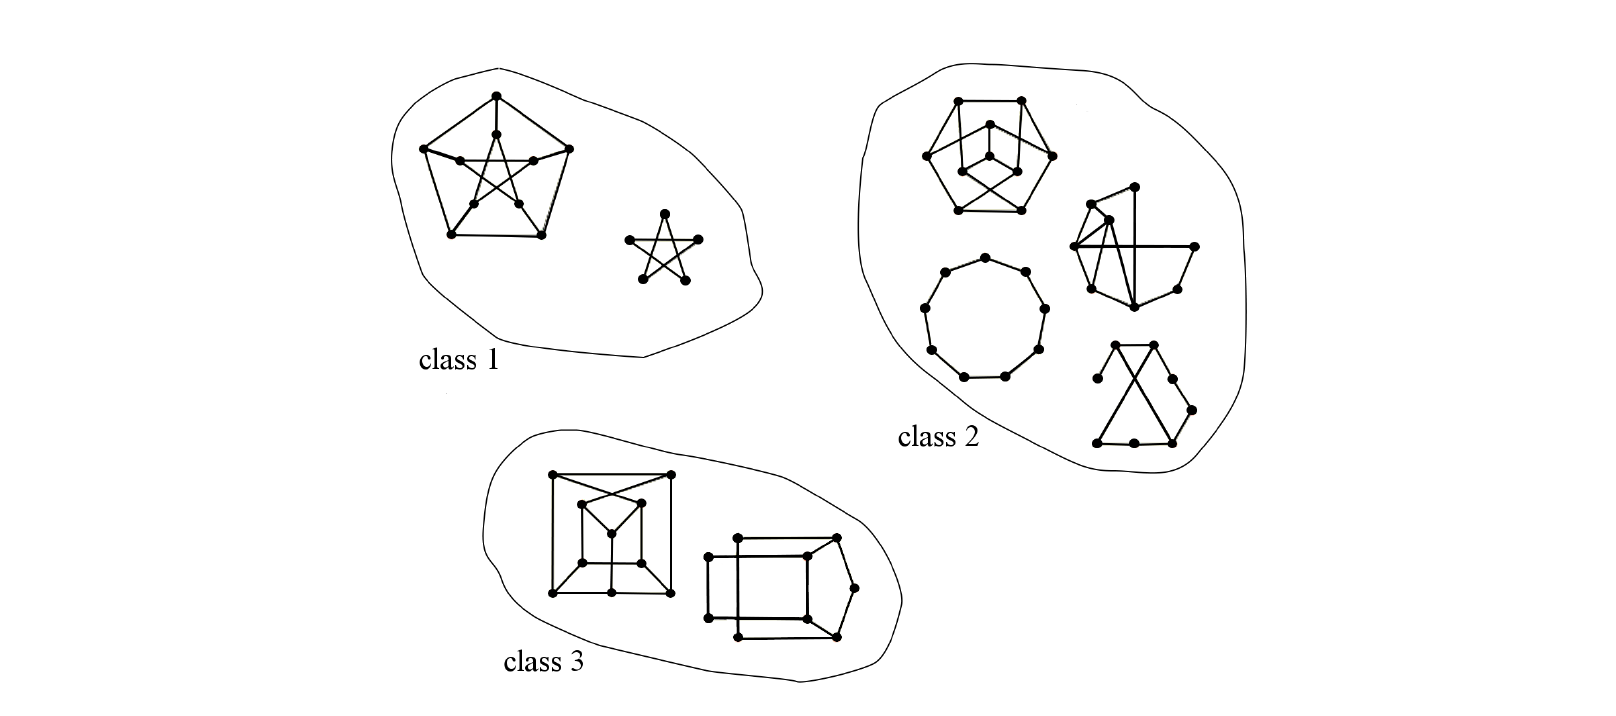
\includegraphics[width=0.95\textwidth,center]{picture/figure6.png}
\caption[Clustering of Graphs]{Clustering of graphs: each of the objects to be clustered is represented by a graph. Source: \cite{Foggia:2014}}
\label{fig:clusteringgraphs}
\end{figure}

\subsection{Graph Kernels}
A graph kernel is a function that maps a few graphs to a real number, and has similar properties to the vector-defined dot product. More formally, if we denote the space of all the graphs with G, a graph kernel is a function k such as:

\begin{equation}
k: \mathbb{G} \times \mathbb{G} \longrightarrow \mathbb{R}
\end{equation}
\begin{equation}
k\left(G_{1}, G_{2}\right)=k\left(G_{2}, G_{1}\right) \quad \forall G_{1}, G_{2} \in \mathbb{G}
\end{equation}
\begin{equation}
\sum_{i=1}^{n} \sum_{j=1}^{n} c_{i} \cdot c_{j} \cdot k\left(G_{i}, G_{j}\right) \geq 0
\end{equation}
\begin{equation}
\forall G_{1}, \ldots, G_{2} \in \mathbb{G}, \forall c_{1}, \ldots, c_{n} \in \mathbb{R}
\end{equation}

In the equation 2.5.3 above, the function k is required to be symmetric, while Equation's 2.5.4 and 2.5.5 respectively requires it to be positive semi-definite. Source: \cite{Foggia:2014}

A graph kernel can be viewed informally as a measure of the similarities between two graphs; however, its formal properties allow a kernel to replace a vector dot product with many vector-based algorithms (and other dot-related functions, such as the Euclidean standard) that use this operator. Thanks to the Mercer theorem, kernels have long been used to extend linear algorithms operating on vector spaces to nonlinear cases: given the kernel function defined on compact Hausdor space X, vector space V and mapping between X and V are used in such a way that the kernel value calculated on two points in X is equal to the dot product of the corresponding points in V. While the theorem of Mercer does not apply to graph kernels, the latter can be used in practice as a theoretically sound way to extend a vector algorithm to graphs. The efficiency of these algorithms, greatly depends on the appropriateness of the notion of similarity expressed within the graph kernel (with relevancy to the task at hand). [\cite{Foggia:2014}] 

[\cite{Kashima:2003}] proposed the concept of marginalized kernels in their paper, a probabilistic approach for defining a kernel based on the introduction of specialized hidden variables for the graph domain. In this case, the hidden variable is a sequence of node indices generated by a random walk on one of the graphs. The sequence kernel is calculated using the sequence of nodes and edges visited given the value of the concealed variable; the marginalized kernel is calculated by estimating the estimated value of the sequence kernel (concerning the combined distribution of the hidden and visible variables). This technique was extended to trees and a molecular data application was presented by [\cite{Mahe:2009}]. To avoid the exponential cost of enumerating all the paths in a graph, the authors proposed using only the shortest path between any pair of nodes because the shortest paths can be calculated in polynomial time. [\cite{Karsten:2005}] proposed a graph kernel based on paths rather than walks (a path is a walk without repeated nodes). In their paper, [\cite{Neuhaus:2006}], they introduced three graph kernels based on Graph Edit Distance. The first kernel necessitates the selection of a zero pattern, a graph that behaves similarly to a null vector with respect to the kernel. The authors discovered that while the kernel meets the theoretical requirements of a kernel function, its functional performance is significantly influenced by the zero pattern selection. The authors then introduced two other kernels derived from the sum and product of the first kernel over a set of zero patterns, and demonstrated that they have the same theoretical properties but are more stable in choosing these patterns.

[\cite{Neuhaus:2009}] in their paper,  presented three possible ways to use Graph Edit Distance in the definition of a kernel. The first way is a diffusion kernel, which transforms the edit distance matrix into a positive definite matrix that satisfies the properties of the kernel, but has the inconvenience that the set of graphs on which it is applied must be finite and known a priori. The second way is a convolution kernel which is based on the decomposition of the edit path between the two graphs into a sequence of substitution operations; this method provides a definition for a kernel between two graphs, given the kernel for individual substitutions. The only downside is the exponential complexity of the number of nodes for which an estimate is proposed by the authors. A random walk kernel is the third way, where the Graph Edit Distance is used to denote a fuzzy graph of the product from which a kernel is obtained that evaluates the local similarity of the corresponding parts of the two graphs.

[\cite{Gauzere:2012:1}] paper introduces two graph kernels. The first is based on the Graph Edit Distance, called the Laplacian Kernel. The operation of the product extracted from the Graph Edit Distance is not guaranteed to be positive definite, and thus does not have the formal properties of the kernel; thus, the authors recommended a technique to obtain a positive definite matrix from the distance matrix, which is then used as the kernel. The second kernel, known as the treelet kernel, is based on treelets, which are all potential trees with less than a fixed number of nodes (up to 6 nodes are considered in the papers); the kernel is determined by counting the occurrences of each treelet in the graphs. Only unattributed graphs can use this kernel, while the Laplacian kernel can also be used for graphs with node and edge attributes. The same authors also later suggested a kernel that is also based on treelets but uses a treelet edit distance instead of merely counting their occurrences to equate the treelets in one graph with those in the other, so as to be tolerant of minor deformations of the graphs. In their article, [\cite{Grenier:2013}]suggested a different treelet-based kernel, especially developed for applications in chemoinformatics, which often integrates knowledge within the graph on the position of each treelet. [\cite{BarbaraStrug:2011}]proposes a kernel based on combining a tree kernel with a classical graph kernel, explicitly developed for hierarchical graphs.